\section{Preliminaries}

In order to fully appreciate the potential applications and programming
patterns used in the Marbles prototype, it is necessary to first go through
some basics of formal tree language theory. In principle, the extension
from string languages is simple - simply allow more than one successor to
each symbol - but obviously this is not sufficiently well-defined to
function very well, formally.

%\subsection{Notation}
%
%Throughout this thesis, unless otherwise specified
%\begin{compactitem}
%\item $\Sigma$ and $\Delta$ will refer to alphabets,
%\item $k,l,n$ and $i$ will refer to integers,
%\item $s, s'$ will refer to symbols,
%\item $q, q', q_1 \ldots q_k$ will refer to states,
%\end{compactitem}

\subsection{Introduction to trees and automata theory}

We define an \emph{alphabet} to be any nonempty set $\Sigma$ of
\emph{symbols}, which can be extended to be a \emph{ranked alphabet}
by adding a mapping $R$ from $\Sigma \rightarrow K \subset N$.

The number $k = R(s)$ we name the \emph{rank} of the symbol $s \in \Sigma$.
We also define the sets $ \forall_{k \in \mathit{range}(R)} \Sigma_k = \{s \in \Sigma \mid R(s) = k\}$
As a convention, we may use a subscript to make the rank explicit, i.e. a
symbol $s$ with rank $R(s) = 2$ may be written $s_2$. Requiring that
symbols have one rank only is not in general necessary, but makes some
proofs and theorems easier to state.

\subsubsection{Trees}

A \emph{tree} can be defined in many ways: as an acyclic graph with a
designated root node or as terms, for example. We persist in moving from a
string perspective, however, and reach this definition:

Let $\{[, ]\}$ be a set of auxiliary symbols, disjoint from any other alphabet considered herein.
The set $T_\Sigma$ of \emph{trees over the (ranked)
alphabet $\Sigma$} is the set of strings defined inductively as follows
\begin{compactitem}
\item for  $a \in \Sigma_0, t = a \in T_\Sigma$
\item for  $a \in \Sigma_k, k \geq 1, t_1 \ldots t_k \in T_\Sigma,  t = a[t_1
\ldots t_k] \in T_\Sigma,$
\end{compactitem}

\begin{figure}[htb]
\center
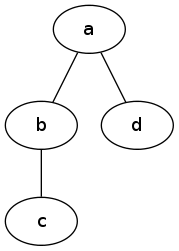
\includegraphics[scale=0.5]{tree.png}
\caption{A simple graphical representation of the tree $a[b[c],d]$}
\label{fig_tree}
\end{figure}

In the tree $t = a[b[c],d]$ (shown graphically in Figure \vref{fig_tree}), the
symbol $a$ is the root of the tree, while $b[c]$ and $d$ are
\emph{child trees}, or \emph{direct subtrees}. The set of all subtrees of a
particular tree, $subtrees(t)$, is composed inductively as follows:
\begin{compactitem}
\item $t$ is in the set $subtrees(t)$
\item if $t'$ is in the set $subtrees(t)$, then all child trees of $t'$ are
in $subtrees(t)$
\end{compactitem}

Further, a tree with no direct subtrees (e.g. $d$), is called a
\emph{leaf}. Thus, $\Sigma_0$ can be seen as a set of trees, as well as a
set of symbols. A \emph{tree language} over $\Sigma$ is any subset of
$T_\Sigma$, again, $\Sigma_0$ serves as an example, namely the tree
language consisting of only leaves.


The \textit{yield} of a tree $t \in T_\Sigma$ is the string over $\Sigma_0$
obtained by reading the leaves of the tree from left to right. 

It should be noted, at this point, that for all trees considered in this
thesis, there is a well-known ordering of the direct subtrees of a tree,
such that each direct subtree can be given an index. However, it is likely
that the complete Marbles system would contain support for unordered trees
as well. 

\subsubsection{String automata}
\label{ssec_fsa}

Recall that a \emph{deterministic finite string automaton (DFSA)} is a
5-tuple $A = (\Sigma, Q, R, F, q_0$, where
\begin{compactitem}
\item $\Sigma$, an alphabet,
\item a set $Q$ of \emph{states}
\item a set $R$ of \emph{rules} on the form
	$q[a] \rightarrow q'$, where $q, q' \in Q$, and $a \in \Sigma$, such
	that each left-hand side occurs at most once, 
\item a set $F \subseteq Q$ of \emph{final states}, and
\item an \emph{initial state} $q_0 \in Q$.
\end{compactitem}

A \emph{configuration} of the DFSA $A$ working on the string $s$ is a 4-tuple
$C = (A, s, q, p)$ where $q \in Q$ is the \emph{current state} of the
automaton and $p \in substr(s)$ is the \emph{position} of the automaton in
the string, defined as the substring that is left to process.

A \emph{run} of a DFSA $A$ on a string $s$ is a sequence $C_0 \ldots C_n$ of
configurations where $A$ and $s$ are the same in each configuration, and
$q_n$ and $p_n$ in $C_n$ relate to $q_{n-1}$ and $p_{n-1}$ in $C_{n-1}$,
and $R$ as follows:
\begin{compactitem}
\item $p_n$ is the substring of $p_{n-1}$ obtained by removing its first symbol
$a$, and
\item there is a rule in $R$ such that
$q_{n-1}[a] \rightarrow q_n$.
\end{compactitem}
\vspace{0.5cm}

An \emph{accepting run} $C_0 \ldots C_n$ of a DFSA $A$ on a string $s$ is run such that
\begin{compactitem}
\item $C_0$ has $q = q_0$ and $p = s$ and
\item $C_n$ has $q \in F$ and $p$ is the empty string
\end{compactitem}
\vspace{0.5cm}

The \emph{regular language accepted by $A$} is the set $L(A)$ of strings on
which accepting runs of $A$ can be constructed.

Further, a DFSA can be seen as a function from the set of strings
$\Sigma^*$ to the boolean values, where every string in the language
results in to \texttt{true}, and every other string to \texttt{false}.

By dropping the requirement that each left-hand side occurs at most in the
rule set, we obtain \emph{non-deterministic finite string automata (NFSA)}.
Configurations for NFSA need to be supplemented only by shifting $q$ from a
single state to a set of states. Runs and accepting runs are supplemented
in a similar fashion. For moving from configuration $C_{n-1}$ to $C_n$, the
relationships between the strings $p_{n-1}$ and $p_n$ and the sets
$q_{n-1}$ and $q_n$ are as follows:
\begin{compactitem}
\item $p_n$ is the substring of $p_{n-1}$ obtained by removing its first symbol
$a$, and
\item for each rule 
$q'_{n-1}[a] \rightarrow q'_n$
in $R$, where $q'_{n-1} \in q_{n-1}$, $q'_n \in q_n$
\end{compactitem}
Similarly, the requirement for an accepting run to have $q \in F$ is
amended such that $q \cap F \neq \emptyset$.

\subsubsection{Tree automata}

While we will more rigorously define tree automata in the next section, a
brief note is in order to explain how string automata are extended to work
on trees. Basically, there are two approaches; Either the automaton has an
initial state which is applied to the root, after which the computation
runs in parallell top-down through the various branches, with the
state-leaf pairs being checked at the end of computation. The alternative
is to have no particular starting state, but instead ''leaf transitions'',
moving from leaf directly to a state, and then working bottom-up through
the tree, culminating in state that is or is not part of the set of final
states. Naturally, these automata exist in deterministic and
non-deterministic versions as well. 

